\dictum[K. Varnalis -- The Guide \emph{(from ``The Light That
  Burns'')}]{ I am not the sow of chance, the forger of new life\\ I
  am a child of necessity, a mature offspring of rage }

\begin{summary}
\item Relational databases are question answering systems that deal
  with information organized in tables or relations.
\item Query optimization and planning revolves around finding an
  efficient algorithm for answering a query.
\item In-memory databases keep all data in main memory so they are
  closer to the processor
\item Many in-memory databases employ some variant of code generation
  to execute the query plans.
\item Intermediate result recycling is the practice of reusing
  computation between queries.
\end{summary}

FluiDB is a system that generally focuses on relational query
optimization and planning. This chapter aims to give the reader some
idea about where FluiDB fits in the design space and the historical
context in which it was developed.  First, we outline a very high
level overview of the \emph{query language and operators} involved in
relational database management systems (RDBMSes) as well as the the overall architecture of such
systems. Following that, we will focus on the \emph{query planning}
subsystems of relational query databases and some traditional
approaches to query evaluation. Afterwards, we will focus particularly
on \emph{in-memory relational databases} and the trade-offs that
govern their design. Finally, we look into the systems that utilize
\emph{intermediate result recycling} and how they solve the problem of
automatically selecting and maintaining intermediate results for
sharing computation within workloads.

\section{Relational databases}

Databases are more than just a method of accessing data. In their
essence they are question answering machines. The typical database
works in a perpetual loop of reading queries and coming up with
answers based on a set of data points. There are two important aspects
that every database needs to define in order to delineate its
operational semantics:

\begin{itemize}
\item The language in which the queries are expressed in
\item The representation of data in terms of which the queries are
  expressed and the results are presented.
\end{itemize}

The oldest, most studied, and most common model is the \emph{relational} model
which defines queries in terms of \emph{relational algebra} and organizes
data in \emph{tables} or relations.

A relation is typically defined as an unordered set of tuples
\(\{d_1,d_2,...,d_k\}\) where each element \(d_i\) represents an
attribute. The core relational algebra is an extension of the algebra
of sets (that defines operators of set union \(\cup\), intersection
\(\cap\), product \(\times\), and difference \(-\)) that includes the
operators of joins \(\Join\), projection \(\pi\) and selection
\(\sigma\). Upon this foundation relational databases typically define
extra operators to increase the expressive power of the language like
aggregations \(\gamma\), semijoins \(\lsemi\), sorting, limiting, etc.

A typical relational database processes operates in a cascading
fashion. It initially receives a query in a textual form. While
relational algebra is the language that underpins the operation of a
relational database, it is rarely the language in which users interact
with it. Instead, most relational databases expect queries written in a
variant of SQL, a query language that is parsed into a tree of
relational algebra operators.

This tree is processed by the query optimizer which rewrites it into a
representation that is efficient to be executed by taking advantage
of the mathematical properties of RA and often gathering statistics
about the underlying data itself. This process leads to the formation
of a relational algebra expression called the \emph{logical plan}. It
is a high level description of a sequence of operations required to
produce a result. A logical plan only assumes the denotational
semantics of these operations, making no assumptions about their
implementation.

Each RA operator is typically implemented by several different
algorithms, each being efficient and even possible in some situations
but not in others. For example, a join can be implemented by nested
loops or by the merge join algorithm, among others.  While the former algorithm is
general and can implement any join, it is very inefficient. On the
other hand a merge join is much more efficient but can only implement
joins of the form \(\Join_{a=b}\) (equijoins or natural
joins). Furthermore, a \emph{logical plan} typically contains only
implied information about the scheduling of the operators, for
example, the logical plan \((\pi A) \Join (\sigma B)\) implies that
the join can not begin being evaluated before the projection and
selection but the latter can be evaluated in any order, or even
simultaneously. All these details about the execution
of the query are resolved by the \emph{physical planner}. The physical
planner accepts a logical plan and emits an unambiguous algorithm that
will produce the result of the query, called the \emph{physical plan}.

The final step is actually executing the physical plan which is
handled by the \emph{query execution engine}. The execution engine
simply evaluates the physical plan on top of the data, making use of
the correct algorithms, auxiliary structures like indexes managing
memory, handling page-level caching, etc.

\section{Query optimization and planning}

\emph{Query optimization and planning} generally is a set of processes that
take place between reading a query and executing a physical plan. The
concerns of query optimization are the correctness of the final result and
the efficiency of the plan generated, usually in terms of time, but
also in terms of space.

Finding an optimal plan is in the general case NP-complete
\cite{ullmanInformationIntegrationUsing1997}, but query optimisers can
do a good job of finding good plans using heuristics. The selection
and organization of these heuristics as well as query cost estimation
are the main problems that make the design of a query optimizer nontrivial. In
particular one could separate the the tasks of a query optimizer
into three broad categories:

\begin{itemize}
\item Query rewriting
\item Query plan enumeration
\item Size and cost estimation (cost model)
\end{itemize}


At a very high level, the architecture of a query optimizer is
demonstrated in figure \ref{fig:optimizer_arch} and is broadly
comprised of the following components:

\begin{figure}[H]
\centering
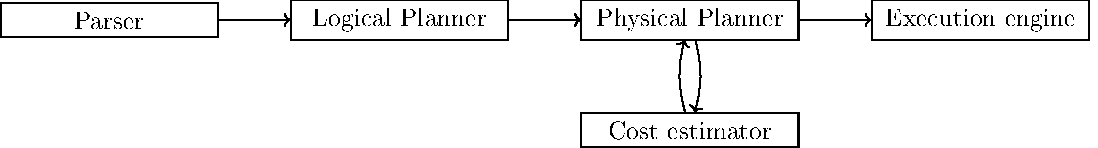
\includegraphics[width=\textwidth]{./imgs/optimizer_architecture.pdf}
\caption{\label{fig:optimizer_arch}Common architecture of a query
  optimizer.}
\end{figure}

\begin{itemize}

\item The \emph{parser} which receives the query in textual form and
  produces a logical plan in the form of an abstract syntax tree.
\item The \emph{deterministic optimizer} or \emph{logical planner}
  that rewrites the logical plan applying optimizations that are based
  solely on the general properties of the relational algebra.
\item The \emph{physical planner} that transforms a logical plan into
  a physical plan that can be unambiguously executed by the execution
  engine to produce a result. The physical planner typically has at
  least some information about the underlying data that the plan will
  operate on like estimations about the statistics of the values or
  the cardinality of the relations.
\item The information about the data being manipulated by the plan is
  inferred by the \emph{cost estimator}. It uses a cost model to
  predict the cost of plans and the cardinality of relations by taking
  into account the provenance of relations as well as physical
  properties of the data like the presence of indexes, the data layout,
  etc.
\end{itemize}

These subsystems are presented here as separate for simplicity and
because in many database systems they are clearly delineated, but it is
also common that they blur into each other. For example, in some RDBMSes
the physical and logical planners are merged into one
\cite{graefeCascadesFrameworkQuery1995,shankarQueryOptimizationMicrosoft2012,solimanOrcaModularQuery2014}. In
fact, it is increasingly common for systems to intersperse query
planning with query execution, adapting the optimization strategy
\cite{graefeDynamicQueryEvaluation1989} to concrete information about
the intermediate results evaluated rather than purely relying on
estimations and predictions
\cite{dingPlanStitchHarnessing2018,chaudhuriPayasyougoFrameworkQuery2008,wuSamplingbasedQueryReoptimization2016,herodotouXplusSqltuningawareQuery2010}. The
degree to which these subsystems are separate is a major concern in
the design space of query optimisers.

Another important aspect to be considered, and which is indeed
important in the design of FluiDB, is the number of queries considered
at a time during optimization and the way in which they are
considered. The optimizer usually considers one query at a time and
maintains little or no state between executions. Although it has found
little adoption in main stream databases, multi-query optimization has
been researched expensively
\cite{michiardiCachebasedMultiqueryOptimization2021,wangMultiqueryOptimizationMapreduce2013,royEfficientExtensibleAlgorithms2000,rogersMultiqueryOptimization2017}. What
is more common in recent years is recycling intermediate
results. RDBMSes that incorporate this technique materialize and cache
intermediate relations, reusing them when they appear as sub-queries
in later queries
\cite{perezHistoryawareQueryOptimization2014,nagelRecyclingPipelinedQuery2013,ivanovaArchitectureRecyclingIntermediates2010}.

The final query processing concern that is relevant to the design of
FluiDB regards the traversal and pruning of the query plan search space. As
mentioned, query optimization is generally NP-complete, so the viable
options DBMS designers are left with are randomized algorithms, ML
approaches, and heuristics. Virtually all systems implement heuristics
entirely or to some degree, while recently more and more also
incorporate randomized algorithms
\cite{chandeGeneticOptimizationJoin2011} and machine learning
\cite{liMachineLearningDatabases2021,marcusNeoLearnedQuery2019}.

\subsection{Logical and physical query optimization}

The \emph{logical planner} transforms a syntax tree in the form of
relational algebraic expressions, where the operators only contain
information about the semantic meaning of the operations and none relating
to, the algorithms that will eventually be executed on the input
data. It is for all intents and purposes a rewrite engine for
relational algebra. Typical transformations performed by the logical
query optimizer are

\begin{itemize}
\item Predicate normalization to conjunctive normal form, e.g.

 \[(a_0 = 1
  \land a_1 = b_1) \lor b_2 = 3 \hookrightarrow (a_0 = 1 \lor b_2 = 3)
  \land (a_1 = b_1 \lor b_2 = 3)\]

\item Predicate push-down e.g. \(A \Join_{a_0 = 1 \land p} B
  \hookrightarrow (\sigma_{a_0 = 1} A) \Join_p B\).
\item Cartesian product to joins \(\sigma_p ( A \times B )
  \hookrightarrow A \Join_p B\)
\item Searching the join ordering space.
\end{itemize}

The \emph{physical query planner}, on the other hand, will specialize
the logical operators deciding on the particular algorithm that should
be used. A physical query planner therefore requires low level
information about the query that relates to the indexes available,
possible ordering of the data, materialized views, etc.

Each of the planners needs to enumerate the plans under
consideration while traversing the search space. There are two major
approaches to this:

\begin{itemize}
\item The \emph{top-down} approach, where the planner establishes the
  top level operator and branches searching the children, backtracking
  as necessary. This was the approach of the descendants of the
  \emph{volcano optimizer} \cite{graefeVolcanoOptimizerGenerator1993a}
  where they implement a "search engine" that uses a branch and bound
  approach to optimization with caching.
\item The \emph{bottom-up} approach where the planner builds and
  connects fragments of a plan accumulating those fragments into a
  larger plan in a traditional dynamic programming approach.
  \cite{raasveldtDuckdbEmbeddableAnalytical2019,kemperHyPerHybridOLTP2011}
\end{itemize}

An important optimizer, on which most modern optimisers are still
being based, is the \emph{cascades optimizer}
\cite{graefeCascadesFrameworkQuery1995}. In short, cascades keeps
track of \emph{groups} of equivalent query expressions and uses those
as the fundamental atom that it manipulates. For example, instead of
keeping track of \(A \Join (B \Join C)\) and \((A \Join B) \Join C\)
separately they would be part of the same query group. Cascades then uses a
global hash table (the "memo" structure) to match the best plan that
corresponds to each group. These plans are stitched together to form larger
plans until the plan for the required query is created in the memo structure.

Many database systems use optimisers similar to cascades (like the
Microsoft SQL server, Postgres,
MemSQL\cite{chenMemSQLQueryOptimizer2016}, and Greenplum -- now Orca
\cite{solimanOrcaModularQuery2014a} to name a few). Notable among the
descendants of cascades is Apache Calcite
\cite{begoliApacheCalciteFoundational2018}, a framework for
implementing query planning used by a number of commercial and
research databases \cite{nunesalonsoBuildingPolyglotData2020}.

% \subsection{Cost estimation}

Probably the hardest aspect of the planner design is the \emph{cost
estimation algorithm}, which is required by the optimisers, especially
the physical planner.  As cost
estimation, we generally refer to a number of different related
procedures that are broadly the \emph{estimation of the cost} of an
arbitrary plan and include the prediction of the \emph{cardinality} of
not yet materialized relations. The role of cost estimation is
detrimental to plan selection and
to the navigation of the plan search space. A good cost model can help basic
planners make decent plans, and a bad one can cause sophisticated
planners make horrible plans \cite{leisHowGoodAre2015}.

It seems that the most important challenges involved in the design of
a cost model relate to the fact that during planning we are fundamentally operating
with sparse and highly uncertain information. Especially relating to
cardinality estimation, uncertainty and bad predictions propagate and
make make it extremely hard for the planners to make correct
decisions. Consider, for example, a join. Some joins are similar to
Cartesian products, producing large output tables, and some joins are
more similar to lookups producing only a few rows. A cost model that
confuses the kind of join will make very bad predictions w.r.t.\ the
cost of any relational algebra expression that uses the said join,
causing an optimizer to select an expensive plan or avoid a cheap
one. What is worse, misestimating the input of an operator caps our
ability to estimate the output.

\begin{comment}
Cardinality estimation most commonly takes the form of selectivity
estimation, i.e., what percentage of tuples from the input make it to
the output of a selection or a join. This is sensitive to the
statistical properties of the values and the selection/join
predicates.

The most common approach is to maintain pre-computed statistics
related to the primary tables. This yields better plans than keeping
no statistics at all, but they are very hard to maintain and their
effectiveness becomes very limited for complex queries. Another
approach employed is to delay the decisions of the optimizer and
essentially merge the planning and plan execution process. This does
not completely eliminate the problem, but it allows the system to have
more up to date and precise data that would allow it to correct course
early in the event of exceptionally bad estimations. One family of
techniques that is becoming popular and was initially used in IBM DB2
\cite{stillgerLEODB2LearningOptimizer2001}, is caching the statistics
of previously computed relations and using that data to make better
predictions in the future. More recently, this takes the form of
employing machine learning to learn from past cardinalities
\cite{ortizEmpiricalAnalysisDeep2019}. This approach is still rarely
used due to the engineering cost of keeping the collected information
up to date.

To give the reader a more well-rounded intuition of the state of cost
estimation besides cardinality estimation, it is worth mentioning that,
to estimate the cost of an operation, Postgres uses magic configurable
variables to weigh IO with CPU evaluation time, while DB2 runs
micro-benchmarks on the production system to make these estimations.

Cost estimation is beyond the current scope of FluiDB and we only
implement the most naive cardinality estimation, but it is worth
mentioning how more mature systems approach the issue.
\end{comment}

\section{In-memory relational databases}

In-memory databases are databases where all data lives in main
memory. The design of in-memory databases is different from the design
of a disk-backed database in a number of respects. To name a few:

\begin{itemize}
\item Page buffers have little use and caching of data in general has very
different goals. While in disk-backed databases caches are mainly used to
avoid disk IO, in in-memory databases they focus on reuse of computation.
\item Concurrency control is much simpler as storage synchronization
concerns are almost entirely eliminated.
\item In disk-backed databases, only a small percentage of time is spend on
actual computation \cite{harizopoulosOLTPLookingGlass2018}. Much of
the non-compute latency is directly linked to the persistent
storage.
\end{itemize}

On the other hand, there are concerns that are specific to the
\emph{lack of backing database storage}. To name a few:

\begin{itemize}
\item Should the system rely on record IDs like in a persistent database
or can it use direct pointers to records?
\item Error prone software can bring the data to an irrecoverable state.
\item Query execution algorithms have fundamentally different
characteristics. While in persistent databases IO dominates the
runtime the bottlenecks for an in-memory database are much more
complex and they can include things like locking, cache misses,
predicate evaluation, and data movements.
\item As main memory is a much less abundant resource than persistent
storage, in-memory databases are often distributed, making network performance a
major concern.
\end{itemize}

One increasingly common technique to address many of these issues,
which is also used by FluiDB, is \emph{code generation}. Since
workloads for in-memory databases are typically CPU bound, there are
major gains in performance to be had by specializing the code being
executed. A typical interpreter-based plan execution engine makes
heavy use of virtual function calls and conditionals inside tight
loops which kills performance on virtually all modern
architectures. The value proposition of code generation is to inline
or hard-code the virtual functions and erase the conditionals at
runtime to reduce the number of operations and make better use of
hardware optimization.

We identify 4 different approaches in the literature to solving this
problem:

\subsection{Transpilation}
\label{sec:transpilation}

Transpilation of a physical plan to a systems language like C or C++
and then fed to an off-the-shelf compiler
\cite{krikellasGeneratingCodeHolistic2010} is expensive but it
generates highly efficient code and more easily debuggable execution
plans. The most notable complete database system that used this
technique were Microsoft Hekaton that generates C code from SQL
queries and older versions of MemSQL. For FluiDB, we reuse many
techniques introduced in HIQUE
\cite{krikellasGeneratingCodeHolistic2010} to translate physical plans
to template-heavy C++ code, making the assumption that query
compilation will be much faster than the query runtime.

\subsection{Third party JIT compilers}

JIT compilation has received a lot of attention in the compiler
community, especially in the context of the JVM. A number of database
systems have taken advantage of this trend to speed up query execution. Most
notable of these are SPARK \cite{armbrustSparkSQLRelational2015}, which
generates Scala AST which is then converted to JVM byte code, and
Neo4j that directly generates bytecode out of the queries.

Systems like Peloton \cite{menonRelaxedOperatorFusion2017} and
recently Postgres \cite{sharyginQueryCompilationPostgreSQL2017}
compile query plans to LLVM IR code that is then passed to the LLVM
compiler to generate high performance machine code. Notable among the
systems that use this approach is HyPer
\cite{neumannEvolutionCompilingQueryEngine} which addresses the
problem of query compilation overhead with an adaptive execution
approach: they built an IR interpreter that starts running the query
while the compiler does proper optimization and compilation of the
LLVM IR program being interpreted. Cheap queries are thus completed
reasonably fast, while in the case of complex queries the interpreted
program is seamlessly replaced by the compiled one once the LLVM
compiler finishes generating machine code.

\subsection{Direct machine code generation}

Some databases do not reuse any compiler or JITing VM, but rather
directly generate highly specific machine code out of the physical
plan. The first system to attempt that, like most techniques used
today, was System-R, which originally compiled SQL statements directly
to machine code by stitching together code fragments from a "fragment
library" \cite{chamberlinHistoryEvaluationSystem1981}. The technique was
quickly deprecated, however, due to the large engineering effort
required. Oracle also includes similar to some of their databases and
MemSQL express their plans in a custom language called MPL (MemSQL
Plan Language) for which they have a custom compiler that translates
it directly to machine code.

\subsection{Custom execution engines}

The final category of databases that use code generation is is per database
code generation rather than per-query code generation. Volcano/EXODUS
\cite{graefeVolcanoOptimizerGenerator1993a} and more recently SageDB
\cite{kraskaSageDBLearnedDatabase} generate an optimizer and execution
engine that is specific to the database schema but not to the queries.
Essentially, these database systems compile the database schema into a
custom RDBMS.

\section{Intermediate result recycling}

A materialized view is a relation defined by a query that is
persistently stored while a view that is not stored is said to be
\emph{virtual}. \emph{View selection} is the process of selecting an
appropriate set of materialized views to improve the performance of a
workload \cite{mamiSurveyViewSelection2012}.  Automated materialized
view selection or intermediate view recycling has occupied
the database research community for a while now. A few approaches to
this problem have to do with AND/OR directed acyclic graphs
\cite{guptaSelectionViewsMaterialize1997}, modeling the problem as a
state optimization \cite{theodoratosDataWarehouseConfiguration1997},
and lattices to represent data cube operations (i.e. multiple
aggregations over the same relation) \cite{ImplementingDataCubes}.

A related problem is \emph{multi-query optimization (MQO)}
\cite{theodoratosDataWarehouseConfiguration1997} that attempts to plan
multiple queries simultaneously. An efficient solution using AND/OR
DAGs was proposed by Roy in
\cite{royEfficientExtensibleAlgorithms2000} where they insert queries
and their sub-queries in a graph and attempt to evaluate a plan by
traversing that graph from multiple sources in a fashion similar to
volcano optimization. Building on that Kathuria
et. al. \cite{kathuriaEfficientProvableMultiquery2017} present an
approximation algorithm that runs in time quadratic to the number of
common subexpressions and provides theoretical guarantees on the
quality of the solution obtained.

Researchers have further looked at opportunistically reusing
intermediate results that would be materialized. Both in traditional
databases
\cite{ivanovaArchitectureRecyclingIntermediates2010,nagelRecyclingPipelinedQuery2013}
and on non-database contexts like MapReduce
\cite{elghandourReStoreReusingResults2012a}, and there have been
attempts to unify the planner with the materialized view selection
engine \cite{perezHistoryawareQueryOptimization2014a}. Notable in this
field is Nectar \cite{gundaNectarAutomaticManagement2010} which is
also not an RDBMS which automatically compresses rarely used data into
programs that generate that data. Nectar focuses on sharing
computation and data as much as possible.

Work such as MRShare \cite{nykielMRShareSharingMultiple2010} tries to
bridge the gap between intermediate result recycling and MQO by
automatically grouping queries in a workload in such a way that
computation can be maximally shared.


\section{Related work}

Our work on FluiDB focuses on intermediate result recycling and query
optimization but on our way to a solution to this particular problem
we had to also work in fields that are fall outside the scope of
database research. In this section we present the prior art in the
three main fields in which the main contributions have been made:

\begin{itemize}
\item Intermediate result recycling (corresponding to chapter 3)
\item Monadic backtracking (corresponding to chapter 4)
\item Incremental computations (corresponding to antisthenis described in
chapter 5)
\end{itemize}

\subsection{Intermediate result recycling}

The fundamental problem being solved by FluiDB falls under the very
general umbrella of \emph{optimizing multiple queries simultaneously}. This
problem is central to database research and there is a very wide
diversity of approaches to solving it. It is useful, however, to
understand this less like a single problem more like a family of
problems. To help the reader understand the philosophy of FluiDB a
high level view we propose an organization of the proposed algorithms
that solve subsets of that problem exist in a space organized around
two poles:

\begin{itemize}
\item The algorithm solves a \emph{set} of queries simultaneously
\item The algorithm solves one query at a time from a \emph{stream} of queries.
\end{itemize}

While many design decisions are informed by the space a piece of work
occupies in relation to this dipole, virtually all approaches involve
identification of common subexpressions or sub-plans that can be
shared between different queries and avoiding duplicate
evaluation. This is indeed the unifying element of the work in the
field.

The former problem has heavily researched for decades and is a major
 subfield in database research \cite{sellisMultipleQueryOptimization1987,royEfficientExtensibleAlgorithms2000,ComputingQueriesDerived}. It's
 focus is slightly narrower as it focuses on identifying common
 subqueries in an unordered set of queries.

The latter (amortized optimization of a \emph{stream} of queries) has also
been dubbed the View Selection Problem (VSP) but research has mostly
focused on static query workloads, i.e. information about the query
workload is known in advance and views are pre-materialized
\cite{phanDynamicMaterializationQuery2008a}. Recently there have been
attempts to mitigate this based on reinforcement learning
\cite{yuanAutomaticViewGeneration2020a} and genetic
algorithms\cite{vijaykumarMaterializedViewSelection2012,zhangGeneticAlgorithmMaterialized1999,bayirGeneticAlgorithmMultipleQuery2007}
due to high volumes, diversity and unpredictability of queries in
modern workloads \cite{liMachineLearningDatabases2021a}. These
approaches have important advantages and shape a field that is rapidly
advances. So far, however, they improve on the heuristics based
solutions. FluiDB's novelty, or at least certain aspects of it, is
orthogonal in that it aspires to reshape the search space of plans, by
introducing the GC and the reversible operations.

On the MQO side, Harizopoulos' two projects StagedDB
\cite{harizopoulosStagedDBDesigningDatabase2005} and QPipe
\cite{harizopoulosQpipeSimultaneouslyPipelined2005} share between
queries that arrive within a time window. This work is seminal and
often cited in the field of MQO.

CJoin \cite{candeaScalablePredictableJoin2009} uses an "always-on" plan
of join operations to execute the joins of all concurrent
queries. Similarly Crescando \cite{giannikisCrescando2010} attempts to
share individual table scans, rather than joins, between queries to
reduce IO. Crescando and other database systems that take similar
approaches, like the aforementioned ones, aim at sharing computation
between temporally overlapping query executions.

DataPath \cite{arumugamDataPathSystemDatacentric2010} creates what they
call a "data-centric approach" to query processing. It transposes the
order in which a per-query system operates (what they call
"computation-centric approach") where the system effectively iterates
over the queries in an outer loop and each query iterates over the
relevant data. Instead DataPath iterates over the data in an outer
loop and an inner loop iterates over the queries looking for a query
that has use for that data. This is a very different approach to the
other but it boils down to sharing data fetches between the queries.

SharedDB \cite{giannikisSharedDBKillingOne2012}, BatchDB
\cite{makreshanskiBatchDBEfficientIsolated2017} and MQJoin
\cite{makreshanskiMqjoinEfficientShared2016a} use a global query plan
for grouped queries. Sloth \cite{cheungSlothBeingLazy2016} CrocodileDB
\cite{shangCrocodileDBEfficientDatabase2020} exploit lazy or deferred
execution to increase the opportunities for batching and therefore
sharing. This way of viewing query planning is conceptually much
closer to FluiDB's approach. In fact the global query plan has many
parallels to the QDAG that we will see in the next chapter. FluiDB,
however, fundamentally differs from these systems as it's aim is
processing streaming queries, rather than requiring ahead of time
knowledge of the entire workload. This leads to radically different
design decisions like reversible queries and the introduction of the
garbage collector.

A slightly more proactive approach is taken by database systems like
MonetDB \cite{idreosMonetdbTwoDecades2012} and CoScan
\cite{wangCoscanCooperativeScan2011} that try schedule queries so
similar or overlapping queries are planned and executed
simultaneously, allowing the system to more easily share computation.

A step closer to the aims of FluiDB is a parallel tradition roughly
started in the 90s by DynaMat \cite{kotidisDynamatDynamicView1999} and
watchman \cite{scheuermannWatchmanDataWarehouse1996} which do dynamic
view selection, choosing which views maintain and which to evict
aiming to reuse them in future queries. These and even more recent
work of view selection focuses on opportunistically reusing
intermediate results that would be materialized
\cite{ivanovaArchitectureRecyclingIntermediates2010,nagelRecyclingPipelinedQuery2013},
taking advantage of tried-and-true optimization techniques that are
however geared towards query at a time processing.

There have been attempts to unify the planner with the materialized
view selection engine like HAWC
\cite{perezHistoryawareQueryOptimization2014a}, which philosophically
is the closest to FluiDB but, in contrast to FluiDB, neither
incorporates a fully specialized optimizer towards nor takes into
account selected views and intermediate results memory requirements
during planning.

Notable in this field is also Nectar
\cite{gundaNectarAutomaticManagement2010} which is not RDBMs. It
automatically compresses rarely used data into programs that generate
that data. Nectar focuses on sharing computation and data as much as
possible.

\subsection{Backtracking and branch-and-bound}

The fundamental framework on which we build our optimizer is a based
on a backtracking monad. Backtracking monads have been researched
quite a bit in the past decades
\cite{kiselyovBacktrackingInterleavingTerminating,hinzeEfficientMonadicstyleBacktracking,hinzeDerivingBacktrackingMonad2000a,fischerReinventingHaskellBacktracking2009}. The
simplest backtracking monad is essentially the list monad which
combined with haskell's lazy semantics amounts simply to nested loops
traversing the search space. More complex search patterns are
introduced by using monad transformers
\cite{hedgesMonadTransformersBacktracking2014} and particularly the
continuation monad transformer
\cite{hinzeMonadicStyleBacktracking1996}. This allows us to jump
between branches (continuations) of the search space. The main problem
being addressed by the literature is that some branches of the search
can be large or infinite. The most popular approach for mitigating
this, other than continuations, comes in the form of interleaving the
execution of different branches via special operators
\cite{kiselyovBacktrackingInterleavingTerminating2005}.

Only recently \cite{kidneyAlgebrasWeightedSearch2021} has prioritized
search been introduced to this area. Since we are able to quantify the
priority of partially constructed query execution plans, this is
fundamentally the approach we require, but we needed from our monad to
support cut-like features. The combination of the latter and weighted
search has, to our knowledge, not been addressed by the literature. In
chapter 4 we present a monad that fits this particular bill.

\subsection{Antisthenis}

An important part of FluiDB is Antisthenis, our highly specialized
incremental computation engine. Incremental computation is in it's
essence an advanced conception of caching. Incremental improvements on
simple memoization techniques
\cite{pughIncrementalComputationFunction1989} have led the modern
notion of self adjusting computation
\cite{acarSelfadjustingComputation2005}. Self-adjusting computation
usually models the computation as a graph of variables and parameters
and focuses on propagating changes of the parameters to the variables
in the graph.

While there has been work on defining general frameworks for
incrementalizing computation like
\cite{hammerAdaptonComposableDemanddriven2014a} and
\cite{andersonEfficientParallelSelfadjusting2021a}, most systems focus
on incrementalizing specific algorithms like
trees\cite{acarDynamizingStaticAlgorithms2004}, kinetic data
structures\cite{acarKineticAlgorithmsSelfadjusting2006}, convex hulls
\cite{acarExperimentalAnalysisSelfadjusting2009}, Huffman
coding\cite{acarTraceableDataTypes2010}, relational databases
\cite{hornIncrementalRelationalLenses2018} and Bayesian inference
\cite{acarAdaptiveBayesianInference2007}.



None of the previous works have unified evaluation strategy with
incremental computation in the context of recursive functions,
particularly ones composed boolean of AND/OR and min/sum operators.

\section{Conclusion}

We presented an overview of the various techniques and challenges of
problems that are directly related to the design of FluiDB and also
some adjacent ones. FluiDB draws inspiration from all these systems to
explore a new approach to managing in-memory data being queried. It
subscribes to the relational model of data and queries and parallels
many techniques introduced for intermediate result recycling and mutli-query
optimization. As an in-memory database, it employs code
generation and takes it to the furthest extreme, generating highly
generic C++ like the HIQUE system, fully compromising on the
performance of the C++ compiler.
